\chapter{Testowanie okienek błędów i innych elementów GUI}
\label{chap:testowanie}

\section{Wprowadzenie}
W tym rozdziale zostaną przedstawione testy przeprowadzone na okienkach błędów oraz innych elementach graficznego interfejsu użytkownika (GUI) aplikacji. Testowanie GUI jest kluczowym etapem w procesie tworzenia oprogramowania, ponieważ pozwala na identyfikację i naprawę błędów, które mogą wpływać na doświadczenie użytkownika.

\section{Okienka ostrzegawcze ekranu logowania}
Okienka ostrzegawcze na ekranie logowania są istotnym elementem interfejsu użytkownika, który informuje o błędach wprowadzonych danych. Testy te mają na celu sprawdzenie, czy okienka poprawnie reagują na nieprawidłowe dane wejściowe.
\begin{figure}[H]
    \centering
    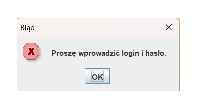
\includegraphics[width=0.8\linewidth]{figures/l1.eps}
    \caption{Brak danych w polach logowania.}
    \label{fig:login_win}
    \small{Źródło: Opracowane przy użyciu Java Swing}
\end{figure}
\clearpage

Podczas testów sprawdzano czy jak ktoś wpisze błędne dane logowania to czy pyta go czy chce się zarejestrować, czy kontynuować logowanie.

\begin{figure}[H]
    \centering
    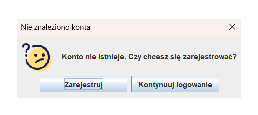
\includegraphics[width=0.8\linewidth]{figures/l2.eps}
    \caption{Błędne dane logowania.}
    \label{fig:login_win}
    \small{Źródło: Opracowane przy użyciu Java Swing}
\end{figure}
\clearpage

\section{Okienka ostrzegawcze ekranu rejestracjii}
Okienka ostrzegawcze na ekranie rejestracji informują użytkownika o błędach wprowadzonych danych podczas tworzenia nowego konta. Testy te mają na celu sprawdzenie, czy aplikacja poprawnie reaguje na nieprawidłowe dane wejściowe, takie jak brak wymaganych pól lub nieprawidłowy format danych.

\begin{figure}[H]
    \centering
    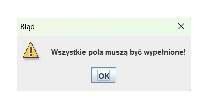
\includegraphics[width=0.8\linewidth]{figures/r1.eps}
    \caption{Brak danych w polach rejestracji.}
    \label{fig:register_win}
    \small{Źródło: Opracowane przy użyciu Java Swing}
\end{figure}
\clearpage

\begin{figure}[H]
    \centering
    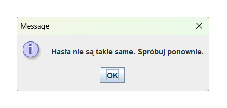
\includegraphics[width=0.8\linewidth]{figures/r2.eps}
    \caption{Sprawdzanie czy hasła są identyczne.}
    \label{fig:register_win}
    \small{Źródło: Opracowane przy użyciu Java Swing}
    \end{figure}
\clearpage

\begin{figure}[H]
    \centering  
    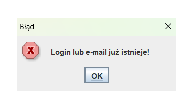
\includegraphics[width=0.8\linewidth]{figures/r3.eps}
    \caption{Sprawdzanie czy login lub e-mail nie są już przez kogoś używane.}
    \label{fig:register_win}
    \small{Źródło: Opracowane przy użyciu Java Swing}
    \end{figure}
\clearpage

\section {Okienka ostrzegawcze ekranu rezerwacji}
Okienka ostrzegawcze na ekranie rezerwacji informują użytkownika o błędach związanych z rezerwacją, takich jak nieprawidłowy format daty lub próba dokonania rezerwacji w przeszłości. Testy te mają na celu sprawdzenie, czy aplikacja poprawnie reaguje na nieprawidłowe dane wejściowe i czy informuje użytkownika o konieczności wprowadzenia poprawnych danych.
\begin{figure}[H]
    \centering
    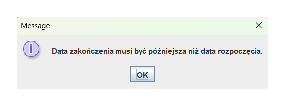
\includegraphics[width=0.8\linewidth]{figures/r4.eps}
    \caption{Data startu rezerwacji jest późniejsza niż końca rezerwacji.}
    \label{fig:reservation_win}
    \small{Źródło: Opracowane przy użyciu Java Swing}
\end{figure}
\clearpage

\begin{figure}[H]
    \centering
    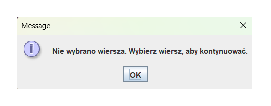
\includegraphics[width=0.8\linewidth]{figures/r5.eps}
    \caption{Nie wybranie wiersza do rezerwacji.}
    \label{fig:reservation_win}
    \small{Źródło: Opracowane przy użyciu Java Swing}   
\end{figure}
\clearpage

\section{Okienka ostrzegawcze ekranu rezerwacji i histori bez logowania}
Okienka ostrzegawcze na ekranie rezerwacji bez logowania informują użytkownika o konieczności zalogowania się, aby móc dokonać rezerwacji. Testy te mają na celu sprawdzenie, czy aplikacja poprawnie reaguje na próby dokonania rezerwacji przez niezalogowanych użytkowników i czy informuje ich o konieczności zalogowania się.

\begin{figure}[H]
    \centering
    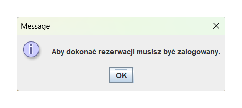
\includegraphics[width=0.8\linewidth]{figures/r6.eps}
    \caption{Próba rezerwacji bez zalogowania.}
    \label{fig:reservation_win}
    \small{Źródło: Opracowane przy użyciu Java Swing}
\end{figure}
\clearpage

\begin{figure}[H]
    \centering
    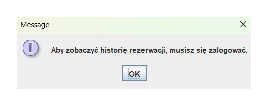
\includegraphics[width=0.8\linewidth]{figures/r7.eps}
    \caption{Próba sprawdzenia historii rezerwacji bez zalogowania.}
    \label{fig:reservation_win}
    \small{Źródło: Opracowane przy użyciu Java Swing}
\end{figure}
\clearpage




